\section{Programs, methods and theory use for development}
\phantomsection

\subsection{Problem Definition}

Nowdays social media become an important marketing tool. Beside a big network where everyone can share information and express their thougts, social media channels represent a good place for advertising different types of products and services. Moreover, people started using social media as a source of helping each others by publishing different advices about how to dress up, how to apply make up and what type of products are good. That is why video blogs that are posting on Youtube are very popular. According to Reasearch Now, 84 \% of people have purchased products based on their descriptions in blogs.\cite{cyber} The percentage is very high, therefore companies are very interested in influential bloggers who can advise their products. 

The problem acquires when stakeholders start researching the influential bloggers. 





\subsection{Big Data}

Every day people around the world post 400 million tweets on Twitter, add 350 million photos to Facebook and view 4 billion videos on YouTube.\cite{digitalInfo} Every 60 seconds on Facebook are posted 510 comments and 293,000 statuses are updated.\cite{zephoria} This has prompted the development of new technical and methodological approache to capture, process and analyse large and complex data, called \textbf{Big Data}. 

A 2011 paper by the McKinsey Global Institute describes big data thus: ``Big data refers to datasets whose size is beyond the ability of typical database software tools to capture, store, manage, and analyze."\cite{bigdata} 

Big data aprroaches to analysing social media data can increase undertanding of how people think and act. Companies can use the information obtained to improve decision-marking, target services and products more effectively and to try to influence users' decisions and behaviours in the future.\cite{POSTNOTE460}

The rate of unstructured data production on social media makes it difficult to analyse and store it using traditional methods. Traditional methods of management system and analytics systems are based on the relational database management system (RDBMS) and can only be applied to structured data.\cite{bdtech} Due to this problem, research community has proposed some solutions that could storage and analyse big data, these solutions and technologies are described in the next subsections.

\subsubsection{Related Technologies}

One of the fundamental technologies related to big data is \textbf{Hadoop}, which forms a powerful big data systematic solution through data storage, data processing, runing applications on clusters and integration of other modules. 

It was initially developed by Doug Cutting and Mike Cafarella as an open-source web search ingine called Nutch. Its purpose was to return web search results faster by distributing data and calculations across different computers so multiple tasks could be acccomplished simultaneously. Later the project was devided - the web crawler part remained as Nutch and the distributed computing and processig part became Hadoop.\cite{sas} Today Hadoop is managed and maintained by the Apache Software Foundation (ASF) and is widely used by big Internet enterprises like Facebook, Yahoo. 


Hadoop consists of two parts: HDFS (Hadoop Distributed File System) and MR framework (MapReduce Framework). HDFS stores data from different external sources fed into a Hadoop cluster. A HDFS cluster includes a single NameNode for managing the metadata of the file system and DataNodes for storing actual data.The MR framework consist of one JobTraker and and multiple TaskTraker nodes.

The described architecture of Hadoop is shown in the \mbox{figure \ref{hdfs_arch}}.

\begin{figure}[!ht]
\centering
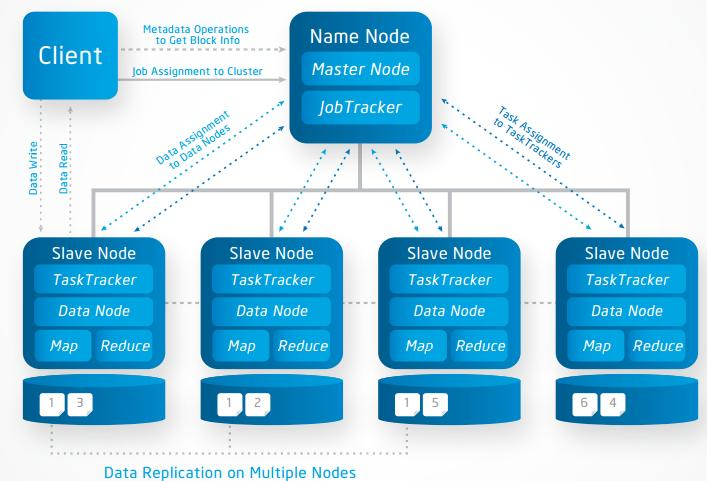
\includegraphics[width=10cm]{hdfs_architecture}
\caption{Hadoop Architecture\cite{hdfsFigure}}\label{hdfs_arch}
\end{figure}

During injection, the data is broken down into smaller chunks. The master node holds all the metadata information regarding the data split up and this enables it to recreate the whole data set using different slave machines.\cite{blog} The client submits a Job to the master node and it in turn assigns the Job to the slave nodes. For assigning the tasks to the salve nodes is respnsible the Jobtracker process that runs on the master node. The task is not run on all the data that is hold on the salve node but only on the data slice that has been specified by the Master Node. The slaves run TaskTracker, HDFS to store data, and map and reduce functions for data computation.\cite{rosebt} If one of the data replicas on HDFS is corrupdet, JobTracker, will look for an alternate slave node that contains the same data. 

MR in complement to a RDBMS is a good fit for problems that need to analyze the whole dataset in a batch fashion and unstructured data. Because, in the case of MR framework, data is partitioned the functional primitives (map and reduce) cand work in parallel on separate partitions. More differences between MR and RDBSMS are shown in \mbox {table \ref{table:mrdiff}}:

\begin{table}[!ht]
\begin{center}
\caption{RDBMS compared to MapReduce \cite{tableHadoop}}
\begin{tabular}{| c | c | c |}
\hline
  & \textbf{Traditional RDBMS} & \textbf{MapReduce} \\
\hline
 \textbf{Data size}& Gigabytes & Petabytes \\
\hline
 \textbf{Access}& Interactive and batch & Batch \\
\hline
\textbf{Updates} & Read and write many times & Write once, read many times \\
\hline
\textbf{Transactions} & ACID & None \\
\hline
\textbf{Structure} & Schema-on-write & Schema-on-read \\
\hline
\textbf{Integrity} & High & Low \\
\hline
\textbf{Scaling} & Nonlinear & Linear \\
\hline
\end{tabular}
\label{table:mrdiff}
\vspace{-2.5em}
\end{center}
\end{table}

The main advantages of Hadoop are:
\begin{itemize}

 \item \textit{High Cost Efficiency} - since large-sclae parallel computing to commercial servers is applied, the cost per terabyte required for storage capacityis greatly reduced.

 \item \textit{Strong Flexibility} - handle many kinds of data from various sources.

 \item \textit{Expandability} - expansion or shrinkage of hardware infrastructure without changing data format.

 \item \textit{High Fault-Tolerance} - recover data and correct computing errors caused by node failures.

\end{itemize}

Having the Hadoop technology which allows to store and analyse big data, the main questions are: Which is the best way of storing the data? What methods are used for data anlysis? 

\subsubsection{Big Data Storage}

Data storage is related to the storage and managemet of large-sclae datasets, while achieving reliability and availability. Storage systems shall be equipped with many interfaces, rapid query, or other type of programming models for analysing of stored data and interaction with it. Traditionally, data storage equipment manages, looks up and analyzes data with structured RDBMSs. But since the volume of the big data is measured in terabytes and petabytes makes traditional storage equipment and management modes inadequate. Therefore, there is a compelling need for research on data storage.\cite{bdtech}

In order develop a large scale distributed storage system for  efficient data processing and analysis the following factors should be taken in consideration:\cite{CAP}

\begin{itemize}

\item \textit{Consistency} - all nodes see the same data at the same time.
\item \textit{Availability} - a guarantee that every request receives a response about whether it succeeded or failed.
\item \textit{Partition tolerance} - the system continues to operate despite arbitrary partitioning due to network failures.

\end{itemize}

In 2000 Eric Brewer proposed a CAP theory, which stated that in a distributed system could not have all this three factors enumerated above simultaneously. The theory was proved two years later by Seth Gibert and Nancy Lynch from MIT. According to the theory we can have a CA system, where partition tolerance is sacrificed, a CP system by ignoring availability and an AP system where consistency element is missing.

\textbf{CA} systems could not handle network failures, because the partition tolerance is missing, this is why they are storage systems with a single server and could not be expanded. So, for large-scale stored systems are used CP systems and AP systems. 

\textbf{CP} systems ensure partition tolerance, in such a way the system can be expanded to become a distributed one. To ensure a level of partition tolerance system maintain several copies of the same data. The copies are completely identical, thus ensuring cosistency. Because CP systems do not have the third factor, availability, to guarantee a response to every request, system will wait for a response from the partitioned node which could reuslt in a timeout error. CP systems are chosen when the amount of data is not so big. Examples of CP systems are: BigTable and Hbase.

\textbf{AP} systems ensure availability and partition tolerance. The consistency factor is missing, therefore AP systems are applied to the scenarios with frequent requests but not very high requirements on accurancy. Availability is also an option when the system needs to continue to function in spite of external errors\cite{AP} for example in online Social Network Services. Two popular AP systems are Dynamo and Cassandra. 









\subsubsection{Big Data Analysis}

